\subsection{Multi-class Object Classification}
% Describe here the CNN architecture.
We use for classification of point cloud data Convolutional Neural Network (CNN).
Our neural network architecture is represented in Figure \ref{fig:cnn}.
The network model is designed for multi-class classification of 
point cloud objects.
% Convolutional neural network provides a promising result of object model with spatial data.
CNN effectively learns the feature recognition of planes, corners, and the edges of the object model.
Our network model is designed with 4 convolutional layers where each layer filter is expected to
recognize planes, corners, edges, and distribution of the objects per orientation.
Other layers learn the global label for the input grid from the knowledge passed by each layer.

\textbf{Input preparation:}
The 3D points \textit{(x,y,z)} of the object are projected into 2D points \textit{(x,y) or (x',y')} (Sec 3.2).
These projected object points are placed on a grid of height 7 and length 10.
This grid is divided into cells of 0.1x0.1 resulting in 70x100 cells and the information about the number of points in each cell is the input to the model.
This input on plotting as pixels will result in the object.

\textbf{Input layer:}
The network model takes a fixed-size input of NxM point counts in grid-cells. We have
used $N=70$ and $M=100$ for our model requirements. The input layer forwards each object input to the 1st layer
of convolutional.


\textbf{Convolutional Layer (input,f,s):}
There are 4 convolutional layers in our architecture to learn features on each orientation.
The first convolutional layer feed on two-dimensional input of size $N \times  M$ from
the input layer, a filter size=f and number of filters=s to be applied.

The filter-size provided to convolutional layer is $5 \times 5$ with 16 such filters to be applied on the input.
The convolutional layer uses filter f to apply convolution operation on input to create a feature map as output.
The convolutional layer learns about the spatial planes, edges, and distribution in the object,
the convolutional layer passes the output to the rectified nonlinearity unit (Relu) before feeding
it forwards to next layers.

\textbf{Max Pooling layer:}
The pooling layer is added to downsample the by a factor of vector d, in
our network model d = [1,2,2,1]. The max pooling layer is after each alternative convolutional
layer, it downsamples the dimension of the feature map with their maximums.

\textbf{Dropout Layer:}
Dropout layer is used for reducing overfitting. As the network is executed on the iterative model with a feed forward network.
The model network tends to overfit on the data. Dropout layer drops random samples from the feature
map.

\textbf{Fully Connected Layer:}
As fully connected layers contain n output neurons. Each neuron of the output is a learned linear
combination of all the outputs from the previous layer, passed through a nonlinearity.
We use ReLUs to save the final output layer, where the number of outputs corresponds
to the number of class labels and a softmax nonlinearity is used to provide a probabilistic output.


% Our Network model starts with an input layer feeding to convolution layer with ReLu then
% another convolutional layer with ReLu and max pool layer then passing input to another batch of convolutional layers
% with Relu and convolutional layer with Relu and max pool, then the feature map is flattened to be feed-forwarded to
% fully connected layer with ReLu, then random samples are dropped with dropout layers
% and finally fed to a fully connected layer and softmax to classify the object into multiclass.

The combination of the above layers is used by some of the state-of-the-art models which have high accuracy on 2-D image inputs.
In order to build the model for this challenge, we have used the above layers, because the input to the model is in the form of pixels.
% Different configurations had different resulted in different models.
%To come up with the state-of-the-art architecture,

\textbf{Model:}
Single objects data is used as input for training the model. We started with implementing a simple 2 layered convolutional neural network,
which uses two convolutional layers with rectified nonlinearity unit and a single layers of the max pool,
drop out and a couple of fully connected layers to classify point cloud objects based upon classes.
This architecture was effective but did not give acceptable results. Further experimenting with layers explained the learning of pixel input by convolutional layer.

The experiment with 4 layered convolutional network has better performance, as they were able to learn planes, edges, and distribution of the point cloud object.
A couple of 2 convolutional layers with alternative Relu added before output and max-pooling layer between them shows the best results while training and testing on individual objects.

The architecture was added with 2 fully connected layers with a single drop out layer to reduce overfitting.
This experimented architecture showed the best result with the training set and the evaluation platform.

\begin{figure*}[!h]
     \begin{center}
       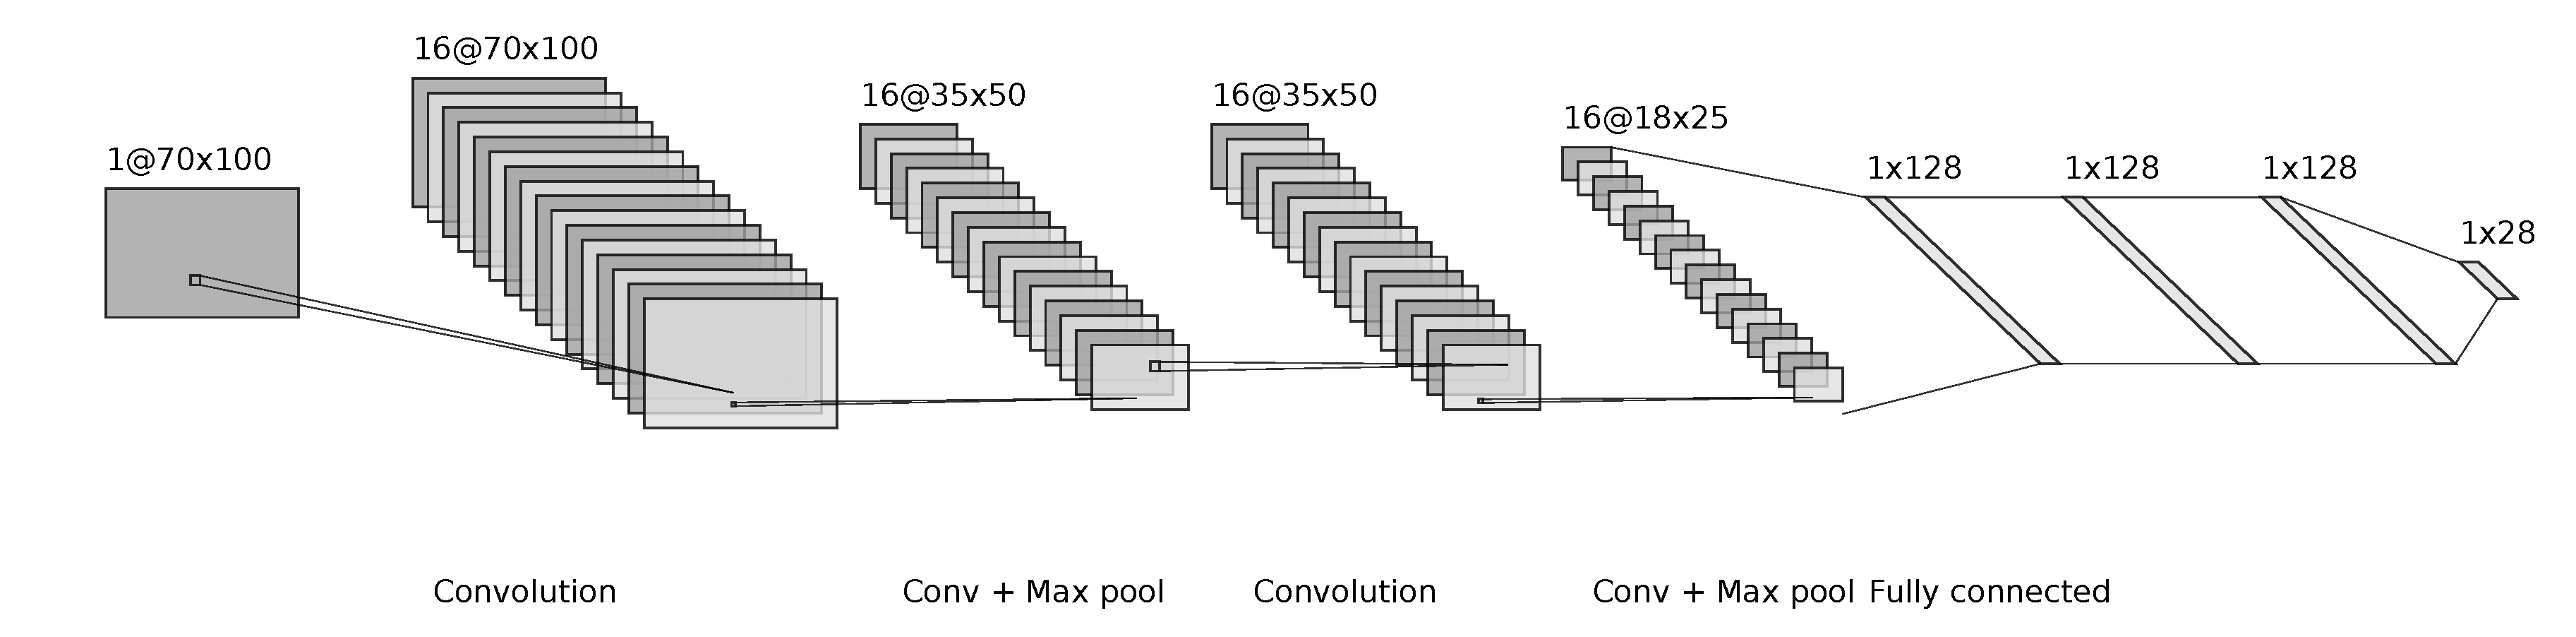
\includegraphics[width=0.8\textwidth]{./images/object_net.pdf}
       \caption{Overview of Convolutional Neural Network Layers with 4 Convolutional Layers}
       \label{fig:cnn}
     \end{center}
\end{figure*}

\subsection{CNN with 3D point cloud Input Data}
We experimented with 3D CNN as dataset could be transformed into the input of 3D CNN being a 3D point cloud dataset.
Our approach was to convert point clouds into a set of voxels by voxelization. Voxelization is the process of conversion of a geometric object from its continuous geometric representation into a set of voxels that best approximates the continuous
object. We used the process to fit a bounding box voxel around the point cloud to form a voxel grid.

We designed for 4 layered 3D CNN architecture with 2 fully connected layers, a dropout layer, around a softmax layer at the end.
The voxel-grid is feed into the network as input and network predict the object out the 28 classes on which network is trained.
The 3D CNN model gave the best performance when trained on a minimal number of class attributes but failed to perform when trained on all the class.
The major reason we tracked for low performance of 3D CNN with a large number of output classes was the density of the object and its distribution.

The performance could be improved by experimenting with lower voxel size to increase more voxels for input.
This method is high resources dependent as the input size grows from several megabytes to several gigabytes, making harder to work on a standard system.
Reviewing the performance between 2D CNN and 3D CNN, the 2D CNN model was providing better performance and precision.
